\documentclass{article}
\usepackage{graphicx} % Required for inserting images
\usepackage{amsmath}
\usepackage{float} 

\title{\textbf{PDM - Assignment1\\}  Graph Search}
\author{Xiaotong Li\qquad 5965373}
\date{November 2023}

\begin{document}
    
    \begin{titlepage}
        \maketitle
    \end{titlepage}
    
    \tableofcontents
    \newpage
    
    \section{Graph Search}
    Consider a directed graph $G = (V, E)$, with distances $d(e)$ for each $e \in E$, and consider two nodes $s, t \in V$. For each node $v$ we define the function $P_s(v)$, which gives the length of the shortest path from $s$ to $v$. Similar we define the function $P_t(v)$, which gives the length of the shortest path from $v$ to $t$.
        \subsection{Question1.1}
        Show that for every edge $e = (u, v)$, the length of the shortest path from node $s$ to node $t$ that uses the edge $e$ is $P_s(u) + d(e) + P_t(v)$.\\\\
        Answer: Since $G$ is a directed graph, so if you want to get to node $t$ via edge $e=(u,v)$ from node $s$, you must first get to node $u$ from node $s$, then get to node $t$ from node $v$. Since $d(e)$ is fixed, it is obvious that the shortest path from $s$ to $t$ is $P_s(u) + d(e) + P_t(v)$.
        \begin{figure}[H]
            \centering
            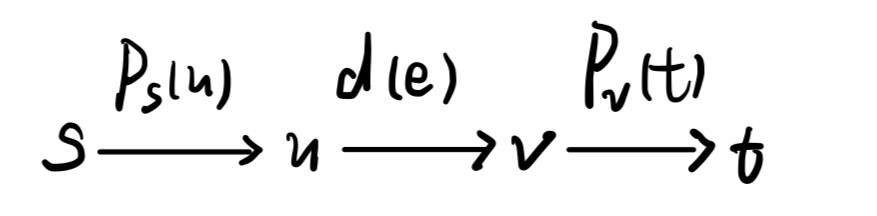
\includegraphics[width=0.5\linewidth]{IMG_EE8351B44859-1.jpeg}
            \caption{Shortest path from $s$ to $t$}
            \label{fig1.1:Shortest path from $s$ to $t$}
        \end{figure}
        \subsection{Question1.2}
        Let $Q$ be the shortest path between the nodes $s$ and $t$. Use the property obtained in Question 1.1, to propose an algorithm that finds the second shortest path from $s$ to $t$ (i.e., considering all paths that are not exactly equal to $Q$)\\\\
        Answer: My algo
    \newpage
    
    \section{Map to Graph}
    \newpage
    
    \section{Dijkstra and A*}
        \subsection{Question3.1}
        \subsection{Question3.2}
        \subsection{Question3.3}
    \newpage
    
    \section{Dijkstra}
        \subsection{Question4.1}
        \subsection{Question4.2}
    \newpage

\end{document}
